% Template for Elsevier CRC journal article
% version 1.2 dated 09 May 2011

% This file (c) 2009-2011 Elsevier Ltd.  Modifications may be freely made,
% provided the edited file is saved under a different name

% This file contains modifications for Nuclear Physics B Proceedings Supplement

% Changes since version 1.1
% - added "procedia" option compliant with ecrc.sty version 1.2a
%   (makes the layout approximately the same as the Word CRC template)
% - added example for generating copyright line in abstract

%-----------------------------------------------------------------------------------

%% This template uses the elsarticle.cls document class and the extension package ecrc.sty
%% For full documentation on usage of elsarticle.cls, consult the documentation "elsdoc.pdf"
%% Further resources available at http://www.elsevier.com/latex

%-----------------------------------------------------------------------------------

%%%%%%%%%%%%%%%%%%%%%%%%%%%%%%%%%%%%%%%%%%%%%%%%%%%%%%%%%%%%%%
%%%%%%%%%%%%%%%%%%%%%%%%%%%%%%%%%%%%%%%%%%%%%%%%%%%%%%%%%%%%%%
%%                                                          %%
%% Important note on usage                                  %%
%% -----------------------                                  %%
%% This file should normally be compiled with PDFLaTeX      %%
%% Using standard LaTeX should work but may produce clashes %%
%%                                                          %%
%%%%%%%%%%%%%%%%%%%%%%%%%%%%%%%%%%%%%%%%%%%%%%%%%%%%%%%%%%%%%%
%%%%%%%%%%%%%%%%%%%%%%%%%%%%%%%%%%%%%%%%%%%%%%%%%%%%%%%%%%%%%%

\documentclass[3p,times,procedia]{elsarticle}

\usepackage{nupha_ecrc}
\usepackage{amsmath}
\usepackage{wrapfig}
\graphicspath{{fig/}}

%% The ecrc package defines commands needed for running heads and logos.
%% For running heads, you can set the journal name, the volume, the starting page and the authors

%% set the volume if you know. Otherwise `00'
\volume{00}

%% set the starting page if not 1
\firstpage{1}

%% Give the name of the journal
\journalname{Nuclear Physics A}

%% Give the author list to appear in the running head
%% Example \runauth{C.V. Radhakrishnan et al.}
\runauth{J.\ Scott Moreland et al.}

%% The choice of journal logo is determined by the \jid and \jnltitlelogo commands.
%% A user-supplied logo with the name <\jid>logo.pdf will be inserted if present.
%% e.g. if \jid{yspmi} the system will look for a file yspmilogo.pdf
%% Otherwise the content of \jnltitlelogo will be set between horizontal lines as a default logo

%% Give the abbreviation of the Journal.
\jid{nupha}

%% Give a short journal name for the dummy logo (if needed)
\jnltitlelogo{Nuclear Physics A}

%% Hereafter the template follows `elsarticle'.
%% For more details see the existing template files elsarticle-template-harv.tex and elsarticle-template-num.tex.

%% Elsevier CRC generally uses a numbered reference style
%% For this, the conventions of elsarticle-template-num.tex should be followed (included below)
%% If using BibTeX, use the style file elsarticle-num.bst

%% End of ecrc-specific commands
%%%%%%%%%%%%%%%%%%%%%%%%%%%%%%%%%%%%%%%%%%%%%%%%%%%%%%%%%%%%%%%%%%%%%%%%%%

%% The amssymb package provides various useful mathematical symbols
\usepackage{amssymb}
%% The amsthm package provides extended theorem environments
%% \usepackage{amsthm}

%% The lineno packages adds line numbers. Start line numbering with
%% \begin{linenumbers}, end it with \end{linenumbers}. Or switch it on
%% for the whole article with \linenumbers after \end{frontmatter}.
%% \usepackage{lineno}

%% natbib.sty is loaded by default. However, natbib options can be
%% provided with \biboptions{...} command. Following options are
%% valid:

%%   round  -  round parentheses are used (default)
%%   square -  square brackets are used   [option]
%%   curly  -  curly braces are used      {option}
%%   angle  -  angle brackets are used    <option>
%%   semicolon  -  multiple citations separated by semi-colon
%%   colon  - same as semicolon, an earlier confusion
%%   comma  -  separated by comma
%%   numbers-  selects numerical citations
%%   super  -  numerical citations as superscripts
%%   sort   -  sorts multiple citations according to order in ref. list
%%   sort&compress   -  like sort, but also compresses numerical citations
%%   compress - compresses without sorting
%%
%% \biboptions{comma,round}

% \biboptions{}


% if you have landscape tables
\usepackage[figuresright]{rotating}

% put your own definitions here:
\newcommand{\trento}{T\raisebox{-0.3ex}{R}ENTo}
\newcommand{\sqrts}{\sqrt{s_\mathrm{NN}}}
\newcommand{\T}{\tilde{T}}

% add words to TeX's hyphenation exception list
%\hyphenation{author another created financial paper re-commend-ed Post-Script}

% declarations for front matter
\usepackage{graphicx}

\begin{document}

\begin{frontmatter}

%% Title, authors and addresses

%% use the tnoteref command within \title for footnotes;
%% use the tnotetext command for the associated footnote;
%% use the fnref command within \author or \address for footnotes;
%% use the fntext command for the associated footnote;
%% use the corref command within \author for corresponding author footnotes;
%% use the cortext command for the associated footnote;
%% use the ead command for the email address,
%% and the form \ead[url] for the home page:
%%
%% \title{Title\tnoteref{label1}}
%% \tnotetext[label1]{}
%% \author{Name\corref{cor1}\fnref{label2}}
%% \ead{email address}
%% \ead[url]{home page}
%% \fntext[label2]{}
%% \cortext[cor1]{}
%% \address{Address\fnref{label3}}
%% \fntext[label3]{}

%% Instructions from Editor: Please use the following \dochead only in the preprint version (e-print arXiv etc.); 
%% use empty \dochead{} when submitting to Nuclear Physics A!
%%\dochead{XXVIth International Conference on Ultrarelativistic Nucleus-Nucleus Collisions\\ (Quark Matter 2017)}
\dochead{}
%% Use \dochead if there is an article header, e.g. \dochead{Short communication}
%% \dochead can also be used to include a conference title, if directed by the editors
%% e.g. \dochead{17th International Conference on Dynamical Processes in Excited States of Solids}

\title{Estimating nucleon substructure properties in a\\
unified model of p-Pb and Pb-Pb collisions}

%% use optional labels to link authors explicitly to addresses:
\author{J.\ Scott Moreland, Jonah E.\ Bernhard, and Steffen A.\ Bass}
\address{Department of Physics, Duke University, Durham, NC 27708-0305}

\begin{abstract}
  We apply a well tested hybrid transport model, which couples viscous hydrodynamics to a hadronic afterburner, to describe bulk observables in proton-lead and lead-lead collisions at \mbox{$\sqrts=5.02$~TeV}.
  The quark-gluon plasma (QGP) initial conditions are modeled using the parametric \trento\ model with additional nucleon substructure parameters to vary the number and size of hot spots inside each nucleon, followed by a pre-equilibrium free streaming stage to match the full energy-momentum tensor of the initial state onto viscous hydrodynamics.
  Initial condition and QGP medium parameters, such as the temperature dependence of the QGP shear and bulk viscosities, are then calibrated using Bayesian parameter estimation to describe charged particle yields, mean $p_T$ and anisotropic flow harmonics $v_2$ and $v_3$ of both collision systems in a single self-consistent framework.
  We find that the hybrid model provides a compelling, simultaneous description of both collision systems using appropriately chosen model parameters, and present new posterior estimates for the size and shape of the nucleon and temperature dependence of QGP shear and bulk viscosities.
\end{abstract}

\begin{keyword}
%% keywords here, in the form: keyword \sep keyword
  Bayesian \sep Flow \sep Initial conditions \sep Quark-gluon plasma \sep Small systems

%% MSC codes here, in the form: \MSC code \sep code
%% or \MSC[2008] code \sep code (2000 is the default)

\end{keyword}

\end{frontmatter}

%%
%% Start line numbering here if you want
%%
% \linenumbers

%% main text
\section{Introduction}

Recently, long-range multiparticle correlations have been observed in high-multiplicity p-Pb collisions which are striking similar to correlations observed in Pb-Pb collisions and commonly attributed to hydrodynamic flow.

These correlations in Pb-Pb collisions are most naturally explained by hydrodynamic flow, a narrative which is evidenced by the global, self-consistent and highly non-trivial agreement of hydrodynamic simulations with experimental measurements.

It is thus natural to wonder if a similar quantitative description of p-Pb bulk observables can be obtained from the hydrodynamic standard model.

The quantitative agreement of hydrodynamic simulations with data remains the strongest evidence for the hydrodynamic picture of heavy-ion collisions.

The justification for the hydrodynamic narrative in heavy-ion collisions

The observation suggests that the so called ``hydrodynamic standard model'', which has been highly successful in modeling the bulk observables of heavy-ion collisions, might also be applied to the small droplets of quark-gluon plasma (QGP) produced in ultracentral p-Pb collisions.

\section{Physics model}

We simulate the QGP initial conditions using a modified version of the \trento\ model \cite{?} which includes parametric nucleon substructure.
Consider the collision of two protons $A, B$ with three-dimensional densities $\rho_{A,B}$ defined as a superposition of Gaussian constituents
\begin{equation}
  \label{density}
  \rho_{A,B}(\textbf{x}) = \sum\limits_{i=1}^{M} \frac{1}{(2 \pi w_c^2)^{3/2}} \exp\left(-\frac{(\textbf{x}-\textbf{x}_i)^2}{2 w_c^2}\right),
\end{equation}
where $M$ is the number of constituents and $w_c$ their Gaussian width.
Here the proton's constituent positions $\textbf{x}_i$ are sampled from a Gaussian radial distribution of width $r=\sqrt{w^2 - w_c^2}$ with free parameter $w$ which varies the ensemble-averaged proton width.

The two protons collide inelastically at impact parameter $b$ with probability
\begin{align}
  \label{pcoll}
  P_\text{coll}(b) = 1 - \exp\left[-\sigma_\text{eff} \int dx\,dy \int dz\, \rho_A(\mathbf{x}) \int dz\, \rho_B(\mathbf{x} + \mathbf{b}) \right],
\end{align}
where $\sigma_\text{eff}$ is a nuisance parameter tuned to fit the total proton-proton inelastic cross section at \mbox{$\sqrts=5.02$~TeV}.
Assuming the protons collide, each is assigned a \emph{fluctuated} participant thickness function
\begin{equation}
  \label{part}
  \T_{A,B}(\mathbf{x}) = \sum\limits_{i=1}^{M} \frac{\gamma_i}{2 \pi w_c^2} \exp\left(-\frac{(\textbf{x}-\textbf{x}_i)^2}{2 w_c^2}\right),
\end{equation}
which integrates out the beam-axis ($\hat{z}$) dimension of Eqn.~\eqref{density} and assigns additional random weights $\gamma_i$ to each constituent sampled from a Gamma distribution with unit mean and variance $1/k^2$.

The \trento\ model then deposits entropy in the proton-proton collision proportional to the generalized mean of participant matter
\begin{equation}
  \label{gmean}
  \frac{dS}{d\eta} \propto \left(\frac{\T_A^p + \T_B^p}{2} \right)^{1/p},
\end{equation}
where the dimensionless parameter $-\infty \le p \le \infty$ modulates the scaling behavior of initial entropy deposition.
The model generalizes readily to proton-lead and lead-lead collisions by calculating the participation probability $P_\text{coll}$ in Eqn.~\eqref{pcoll} for all pairs of colliding nucleons and summing the fluctuated participant thickness function $\T_{A,B}$ in Eqn.~\eqref{part} over all participants.

We use Eqn.~\eqref{gmean} to generate boost invariant initial conditions for p-Pb and Pb-Pb collisions at $\sqrts=5.02$~TeV, and free stream the initial profiles for proper time $\tau_{fs}$.
The full energy-momentum tensor is then matched to the \texttt{VISH2+1} hydrodynamics code which includes shear and bulk viscous corrections in the 14-moment approximation.
The hydrodynamic evolution is subsequently matched to a microscopic Boltzmann transport model along a pre-specified switching isotherm $T_\text{sw}$, treated as a free parameter.
We sample particles from the Cooper-Frye formula with shear and bulk viscous corrections to the distribution function \ref{?}, and simulate subsequent hadronic interactions using the \texttt{UrQMD} microscopic transport model.
Finally, we calculate hadronic observables on the particles using the same kinematic cuts and methods used by experiment.

\section{Model calibration}

%which computes the density of participant matter in each nucleus from Glauber cross sections, and parametrizes local entropy deposition using a flexible functional form known as the generalized mean,
%\begin{equation}
%  dS/d\eta \propto \left(\frac{\T_A^p + \T_B^p}{2}\right)^{1/p}
%\end{equation}
%where the participant thickness functions $\T_{A,B}$ denotes the beam integrated density of participant matter in nucleus A and B respectively.
%



%\begin{figure}
%  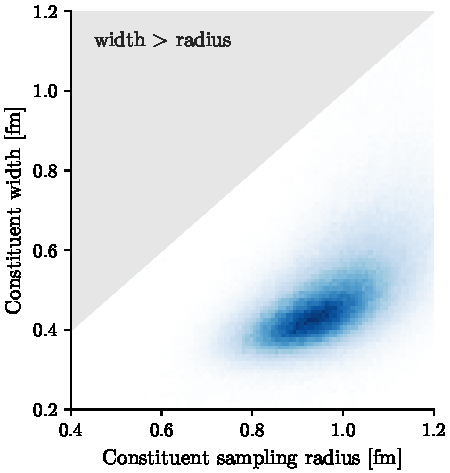
\includegraphics{proton_posterior_shape}
%  \caption{\label{fig:proton_shape}
%  }
%\end{figure}

\section{Results}

%% References
%%
%% Following citation commands can be used in the body text:
%% Usage of \cite is as follows:
%%   \cite{key}         ==>>  [#]
%%   \cite[chap. 2]{key} ==>> [#, chap. 2]
%%

%% References with BibTeX database:

\bibliographystyle{elsarticle-num}
\bibliography{proceeding}

%% Authors are advised to use a BibTeX database file for their reference list.
%% The provided style file elsarticle-num.bst formats references in the required Procedia style

%% For references without a BibTeX database:

%\begin{thebibliography}{00}
%
%% \bibitem must have the following form:
%%   \bibitem{key}...
%%
%
%\bibitem{jonah_mtd}
%
%\end{thebibliography}

\end{document}

%%
%% End of file `nupha-template.tex'.
